\documentclass[12pt,a4paper,twocolumn]{article}

\usepackage[english]{babel} 		%% englische Sprache

\usepackage[latin1,applemac]{inputenc}	%% deutsche Umlaute wie normale
 					%% Buchstaben verwenden 
 					%% (ansonsten muesste � durch a getippt werden)
\usepackage{a4wide} 			%% kleinere Seitenr�nder

\usepackage{amssymb,amsthm,amsfonts, amsmath}
								%% diverse Matheerweiterungen, z.B. \implies
 								%% diverse Matheerweiterungen, z.B. \mathbb{R}
%\usepackage{stmaryrd} 			%% weitere Symbole
\usepackage{epsfig} 			%% um eps-Dateien einzubinden (\epsfig{file=...})
\usepackage{longtable} 			%% fuer Tabellen ueber mehrere Seiten
\usepackage{color}
\usepackage{hyperref}
\usepackage{dsfont}
\usepackage{caption}
\usepackage{multirow}

\title{ \textit{Some super concise and informative title} \\ Data Analysis Project for \\ \textit{Machine Learning: Basic Principles}}
%\author{H�ctor Laria Mantec�n and Maximilian Proll}
\date{\today}

\begin{document}

\maketitle

\begin{abstract}

\textit{
Precise summary of the whole report, previews the contents and results. Must be a single paragraph between 100 and 200 words.
}

\end{abstract}

\section{Introduction}

\textit{
Background, problem statement, motivation, many references, description of contents. Introduces the reader to the topic and the broad context within which your research/project fits
\begin{itemize}
\item What do you hope to learn from the project?
\item What question is being addressed?
\item Why is this task important? (motivation)
\end{itemize}
Keep it short (half to 1 page).
}

\section{Data analysis}
This competition is performed on two datasets, a training and a test dataset with $4.363$ resp. $6.544$ songs. Each dataset has a total of $264$ features, which will be used for predicting one of $10$ classes. The features con be grouped into the 3 main components of music: timbre, pitch and rhythm. The $10$ classes are:  Pop Rock, Electronic, Rap, Jazz, Latin, R\&B, International, Country, Reggae and Blues.

In order to better visualise the training data we performed the \textit{t-Distributed Stochastic Neighbor Embedding} (\textbf{t-SNE}) with $3$ remaining dimensions. The result of this award-winning embedding is shown below:

\begin{center}
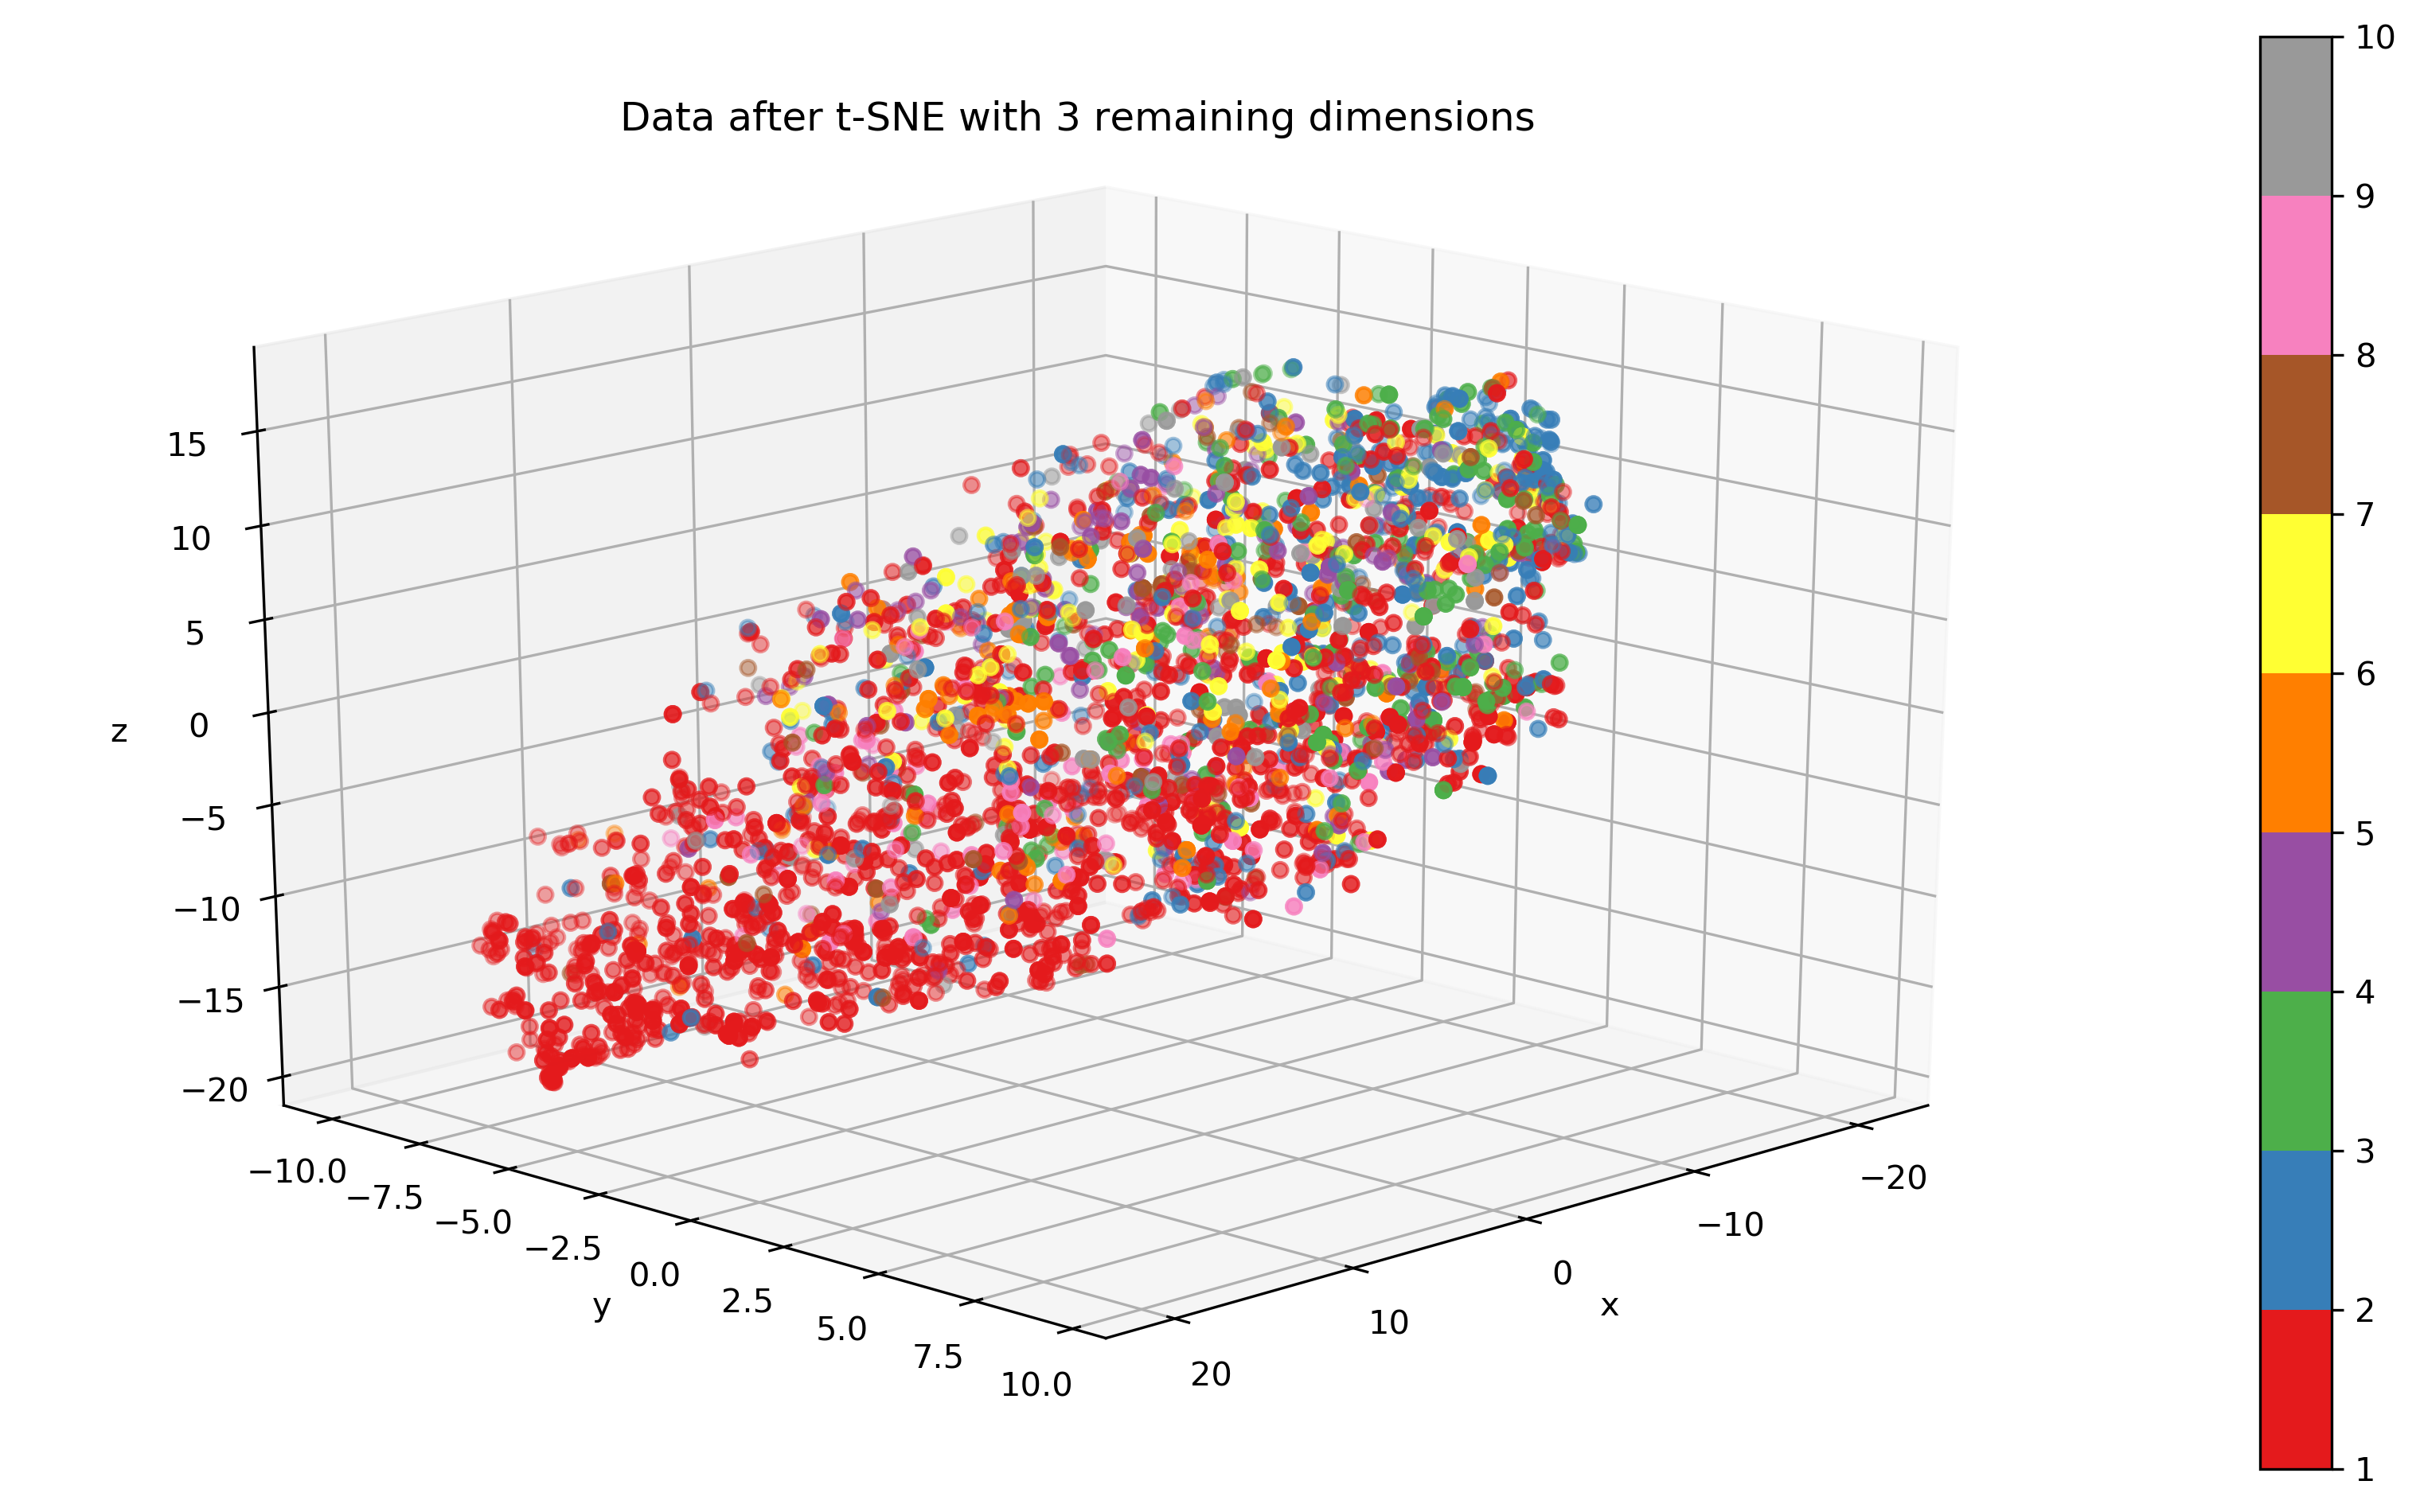
\includegraphics[width=\linewidth]{report_files/TSNE_data.png}
\end{center}

It is also important to know the distribution of the given training dataset. The distribution is shown in the following picture:

\begin{center}
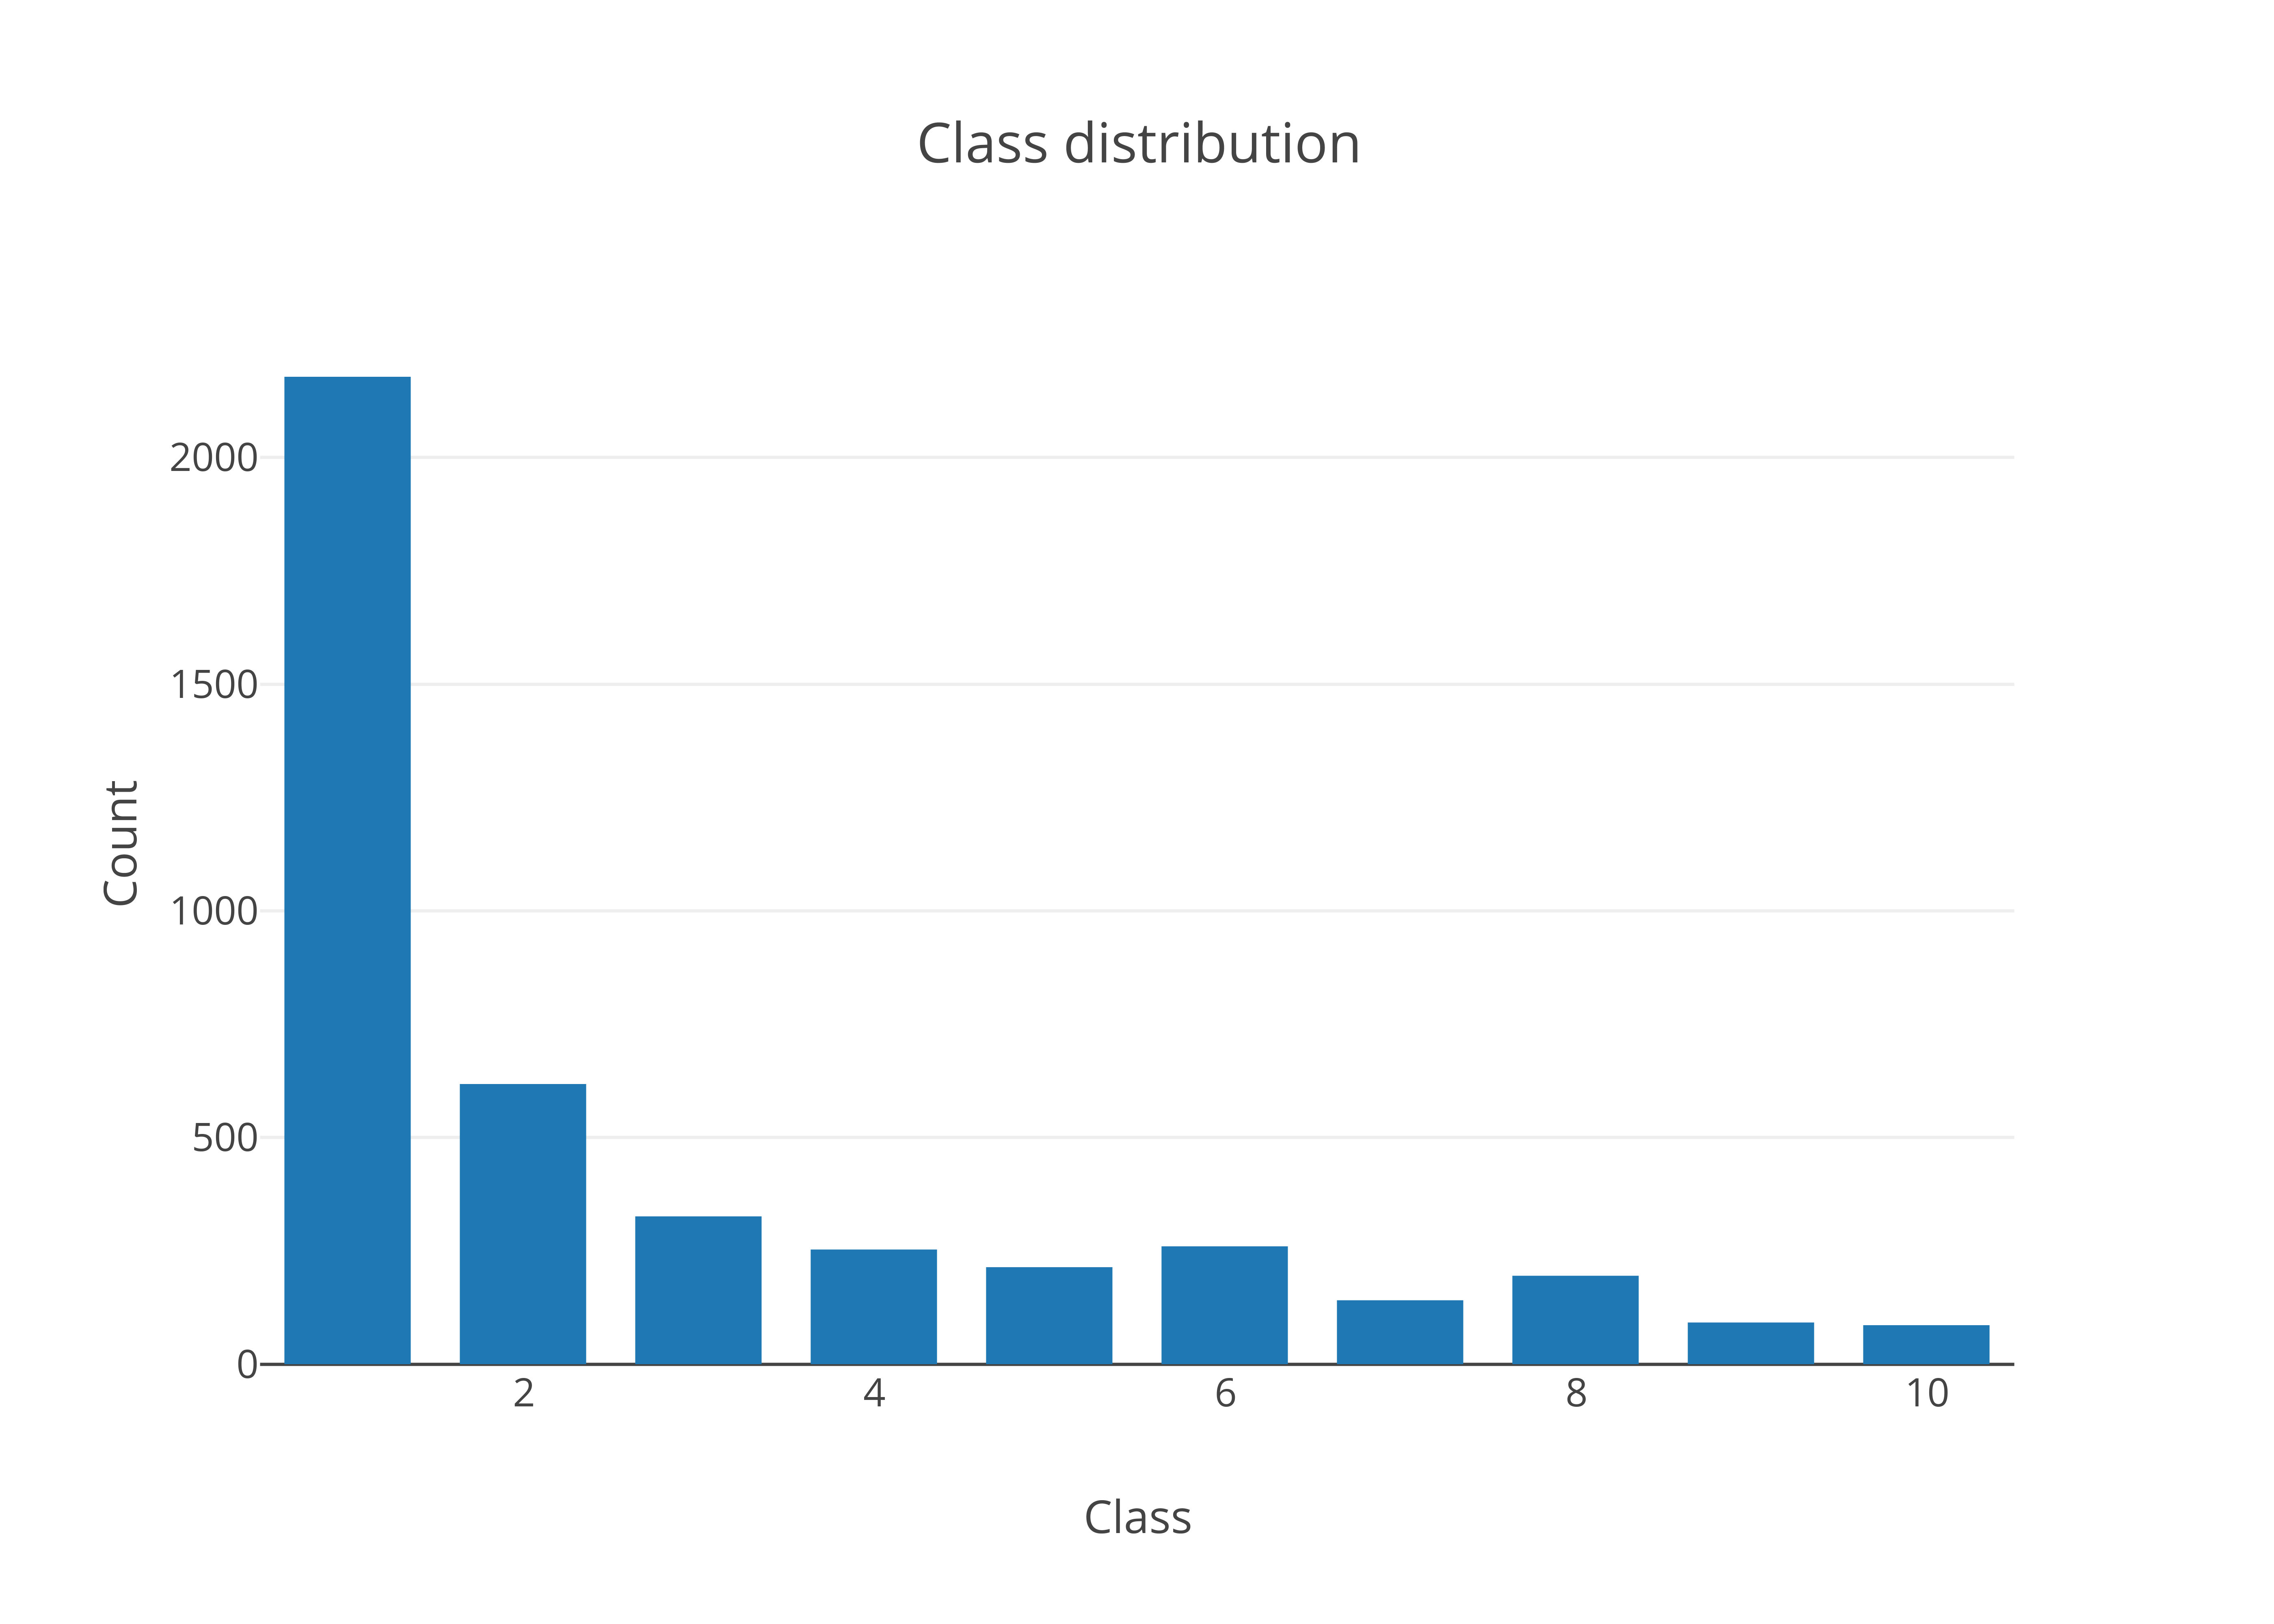
\includegraphics[width=\linewidth]{report_files/Class_distribution.png}
\end{center}

This distribution shows very clearly that the training data is skewed, which means that the predictor will be able to generalise better for the majority classes.

%in case we need to fill more space we could add a boxplot of the 264 features.


%\textit{
%Briefly describe data (class distribution, dimensionality) and how will it affect classification. Visualize the data. Don�t focus too much on the meaning of the features, unless you want to.
%\begin{itemize}
%\item Include histograms showing class distribution.
%\end{itemize}
%}

\section{Methods and experiments}

\textit{
Explain your whole approach (you can include a block diagram showing the steps in your process).
\begin{itemize}
\item What methods/algorithms, why were the methods chosen.
\item What evaluation methodology (cross CV, etc.).
\end{itemize}
}

\subsection{Logistic Regression}

\subsection{Support Vector Machines}

\subsection{Naive Bayes}

\subsection{Neural Networks}
For this approach, we tried a fixed architecture of 5 layers with 100 to 200 units but different setting of hyper-parameters. 

\section{Results}

\textit{
Summarize the results of the experiments without discussing their implications.
\begin{itemize}
\item Include both performance measures (accuracy and LogLoss).
\item How does it perform on kaggle compared to the train data.
\item Include a confusion matrix.
\end{itemize}
}

We can see measurements of the methods chosen in Table~\ref{table:measurements}.

\begin{table}[h]
\centering
\caption{Performance measurements (accuracy and LogLoss), and performance on Kaggle competition.}
\label{table:measurements}
\begin{tabular}{llcc}
                                  &         & \textbf{Validation} & \textbf{Kaggle} \\ \hline
\multirow{2}{*}{\textbf{Log Reg}} & Accuracy  & 0.74329             & 0.65021         \\ \cline{2-2}
                                  & Log. Loss & -                   & 0.17736         \\ \hline
\multirow{2}{*}{\textbf{SVM}}     & Accuracy  & 0.85835             & 0.60238         \\ \cline{2-2}
                                  & Log. Loss & -                   & 0.25370         \\ \hline
\multirow{2}{*}{\textbf{NB}}      & Accuracy  & -                   & 0.61720         \\ \cline{2-2}
                                  & Log. Loss & -                   & 0.19949         \\ \hline
\multirow{2}{*}{\textbf{NN}}      & Accuracy  & 0.73779             & 0.63523         \\ \cline{2-2}
                                  & Log. Loss & -                   & 0.19893         \\ \hline
\end{tabular}
\end{table}

\section{Discussion/Conclusions}

\textit{
Interpret and explain your results
\begin{itemize}
\item Discuss the relevance of the performance measures (accuracy and LogLoss) for
imbalanced multiclass datasets.
\item How the results relate to the literature.
\item Suggestions for future research/improvement.
\item Did the study answer your questions?
\end{itemize}
}

\section{References}

\textit{List of all the references cited in the document
}

\section{Appendices}

\textit{Additional information that is not essential to explain your findings, but supports your work. For example, source code, additional images, mathematical derivations, etc.
If you include source code, don�t include the whole code, focus only on the most important parts, for example, a function implementing a specific algorithm
}


\end{document}